\chapter{Дополнительные замечания о системе NorthStar}\label{app_about_ns}
Опыт работы с системой NorthStar в рамках учебных проектов и настораживающие объяснения, касающиеся ее работы в официальной документации\lefteqn{,}\footnote{В~\cite[стр.~30--31]{northstar_manual} о точности системы говорится только в контексте повторного достижения роботом позиции, координаты которой уже были предварительный найдены с помощью системы NorthStar.
Очевидно, что из данных объяснений нельзя сделать какие-либо выводы о точности определения координат робота на полу в принципе.}
заставили усомниться в правильности возвращаемых системой данных.

Для проверки этих подозрений был поставлен ряд экспериментов.
Их описание и полученные результаты~--- см.~Приложение~\ref{app_expers_with_ns}.
Дополнительно к сказанному там можно добавить лишь следующее.

Как можно видеть на представленных в упомянутом приложении рисунках, отражающих характер экспериментальных данных, последние подвергнуты искажениям.
К~примеру <<сетка>> экспериментальных данных, показанная на рисунке~\ref{img_second_result_of_exps}, <<загнута>> сверху и снизу.
Иначе говоря, вдоль вертикальной оси рисунка она подвержена искажениям, подобным тем, которые возникают на фотографиях при наличии у оптической системы фотокамеры дисторсии\lefteqn{.}%
\footnote{Надо сказать, что подобные искажения наблюдались и в остальных экспериментах с системой NorthStar.}
При таких условиях естественно может возникнуть желание провести какие-нибудь количественные исследования этих искажений и, возможно, даже как-то попытаться их исправить.
В~таком случае при постановке экспериментов, подобных описанным в Приложении~\ref{app_expers_with_ns}, рекомендуется, во-первых, проводить их в пустом помещении, чьи размеры в обоих измерениях существенно больше, чем $6\times6$~м\lefteqn{,}%
\footnote{Эксперименты, описанные в Приложении~\ref{app_expers_with_ns} проводились в помещении, имеющем размер $6\times8$~м.}
(это позволит исключить из результатов искажения, вызываемые окружающими предметами), а во-вторых, для выравнивания системы координат СКП и экспериментальной разметки использовать метод, описанный в Приложении~\ref{app_expers_with_ns_2}.



\chapter{Описание проверяющих работоспособность системы NorthStar экспериментов}\label{app_expers_with_ns}
Для проверки работоспособности системы NorthStar были выполнены следующие действия:
\begin{enumerate}
	\item на предмет выяснения роли, которую играет калибровочный коэффициент, и внутренних механизмов вычисления координат, был изучен исходный код ПО, управляющего работой Robotino и отвечающего за снятие данных с системы NorthStar;
	\item проверен факт идентичности данных, возвращаемых парой использованных в работе приемников NorthStar;
	\item проверена гипотеза о том, что положение начала системы координат, относительно которой возвращаются координаты приемника, находится в точке, в которую проецируется на пол с потолка центр отрезка, ограниченного видимыми точками красного цвета;
	\item проверена гипотеза о том, что положение оси ординат системы координат, относительно которой возвращаются координаты приемника, есть прямая, на которой лежит проецируемый на пол с потолка отрезок, ограниченный видимыми точками красного цвета;
	\item исследован характер искажений в возвращаемых системой данных.
\end{enumerate}

Комментируя каждое из этих действий более подробно, можно сказать следующее.

В результате выполнения первого из них, во-первых, были выяснены внутренние механизмы вычисления системой NorthStar координат приемника (ошибок в соответствующих вычислениях не обнаружено), а во-вторых, был установлен смысл коэффициента, который необходимо настраивать при калибровке.
Последний в изменениях возвращаемых системой NorthStar координат оказался играющим роль обычного коэффициента пропорциональности (см.~в ссылке на SVN c \cite{wiki_openrobotino} файл \verb|/common/trunk/lib/rec/nstar2/Report.h|).

Второй из указанных экспериментов, состоящий из следующих шагов:
\begin{enumerate}
	\item включить и откалибровать систему;
	\item поставить первого Robotino, оборудованного первым приемником, в произвольную точку и запомнить координаты, выдаваемые при этом системой NorthStar;
	\item поставить  второго Robotino, оборудованного вторым приемником, в ту точку, в которой стоял первый Robotino, и сравнить получаемые данные с записанными на прошлом шаге;
	\item в~случае совпадения данных из двух прошлых пунктов повторить описанные в них действия еще несколько раз для подтверждения успеха; в случае несовпадения остановиться на данном этапе и выяснить, чем это может быть вызвано.
\end{enumerate}
подтвердил идентичность c точностью до нескольких сантиметров возвращаемых приемниками данных.
Пример полученных результатов см.~на рисунке~\ref{img_sameless_exps}.

\begin{figure}[h!]
	\centering
	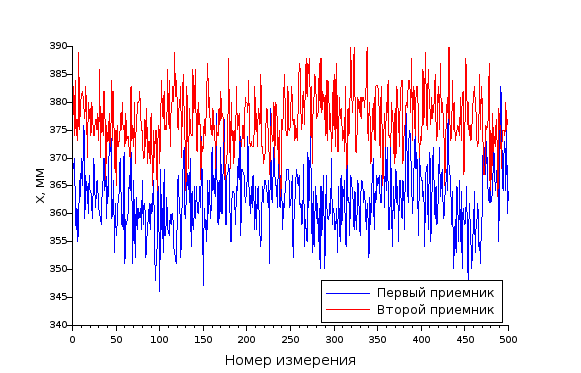
\includegraphics[height =10cm]{example_of_ns_x.png}
	\caption{Пример выдаваемых приемниками сигналов, содержащих информацию об абсциссах роботов.}
	\label{img_sameless_exps}
\end{figure}

Третье из названных выше действий также подтвердило соответствующую гипотезу.
Всего его реализация состояла из следующих этапов:
\begin{enumerate}
	\item подключить и откалибровать систему NorthStar;
	\item активировать излучение проектором на потолок видимых точек красного цвет;
	\item найти центр ограниченного ими отрезка на потолке (для этого один из проводящих эксперимент людей должен был залезть на стремянке до потолка с рулеткой и выполнить эту операцию простым измерением);
	\item опустить из найденной точки отвес;
	\item в точку на полу, на которую он укажет, поставить Robotino и убедиться, что координаты последнего составят пару $(0; 0)$;
	\item в случае успеха повторить описанные действия еще два-три раза.
\end{enumerate}

Результаты выполнения четвертой из поставленных задач также показали справедливость выдвинутой для проверки гипотезы.
Конкретные шаги, проделанные для этого, даются таким списком:
\begin{enumerate}
	\item отметить по описанной ранее технологии положения на полу проекций на него с потолка красных видимых точек, создаваемых излучателем;
	\item поместить по очереди в них Robotino и убедится, что его нахождение в этих точках будет описываться разными ординатами (при этом они будут равны по модулю, но противоположны по знаку) и одинаковыми и предельно близкими к нулю абсциссами.
\end{enumerate}

Самый последний пункт в перечне необходимых дел состоял из следующих действий:
\begin{enumerate}
	\item подключить и откалибровать систему NorthStar;
	\item разметить на полу квадрат, состоящий из $11{\times}11$ точек, расстояние между координатами которых 40~см (см.~рисунок~\ref{img_expers_quadro});
	\item \label{item:alignment}Поместить проектор системы Northstar, чья голова приблизительно направлена вертикально вверх, в точку 0, примерно выравнивая отрезок, ограниченный на потолке точками, создаваемыми проектором, параллельно одной из сторон размеченного квадрата;
	\item поместить одного из Robotino в каждую обозначенную на полу точку и зафиксировать его координаты, полученные с NorthStar, в ней; при этом в качестве его координат стоит взять среднее из, например, 10 возвращаемых значений (данное требование необходимо по той причине, что, как можно видеть из рисунка~\ref{img_sameless_exps}, получаемые с NorthStar сигналы зашумлены);
	\item повторить описанные в прошлом пункте действия еще раз;
	\item повторить все описанные в двух прошлых пунктах действия для второго из роботов и при повороте проектора на 90 градусов, относительно вертикальной оси;
\end{enumerate}

\begin{figure}[h!]
	\centering
	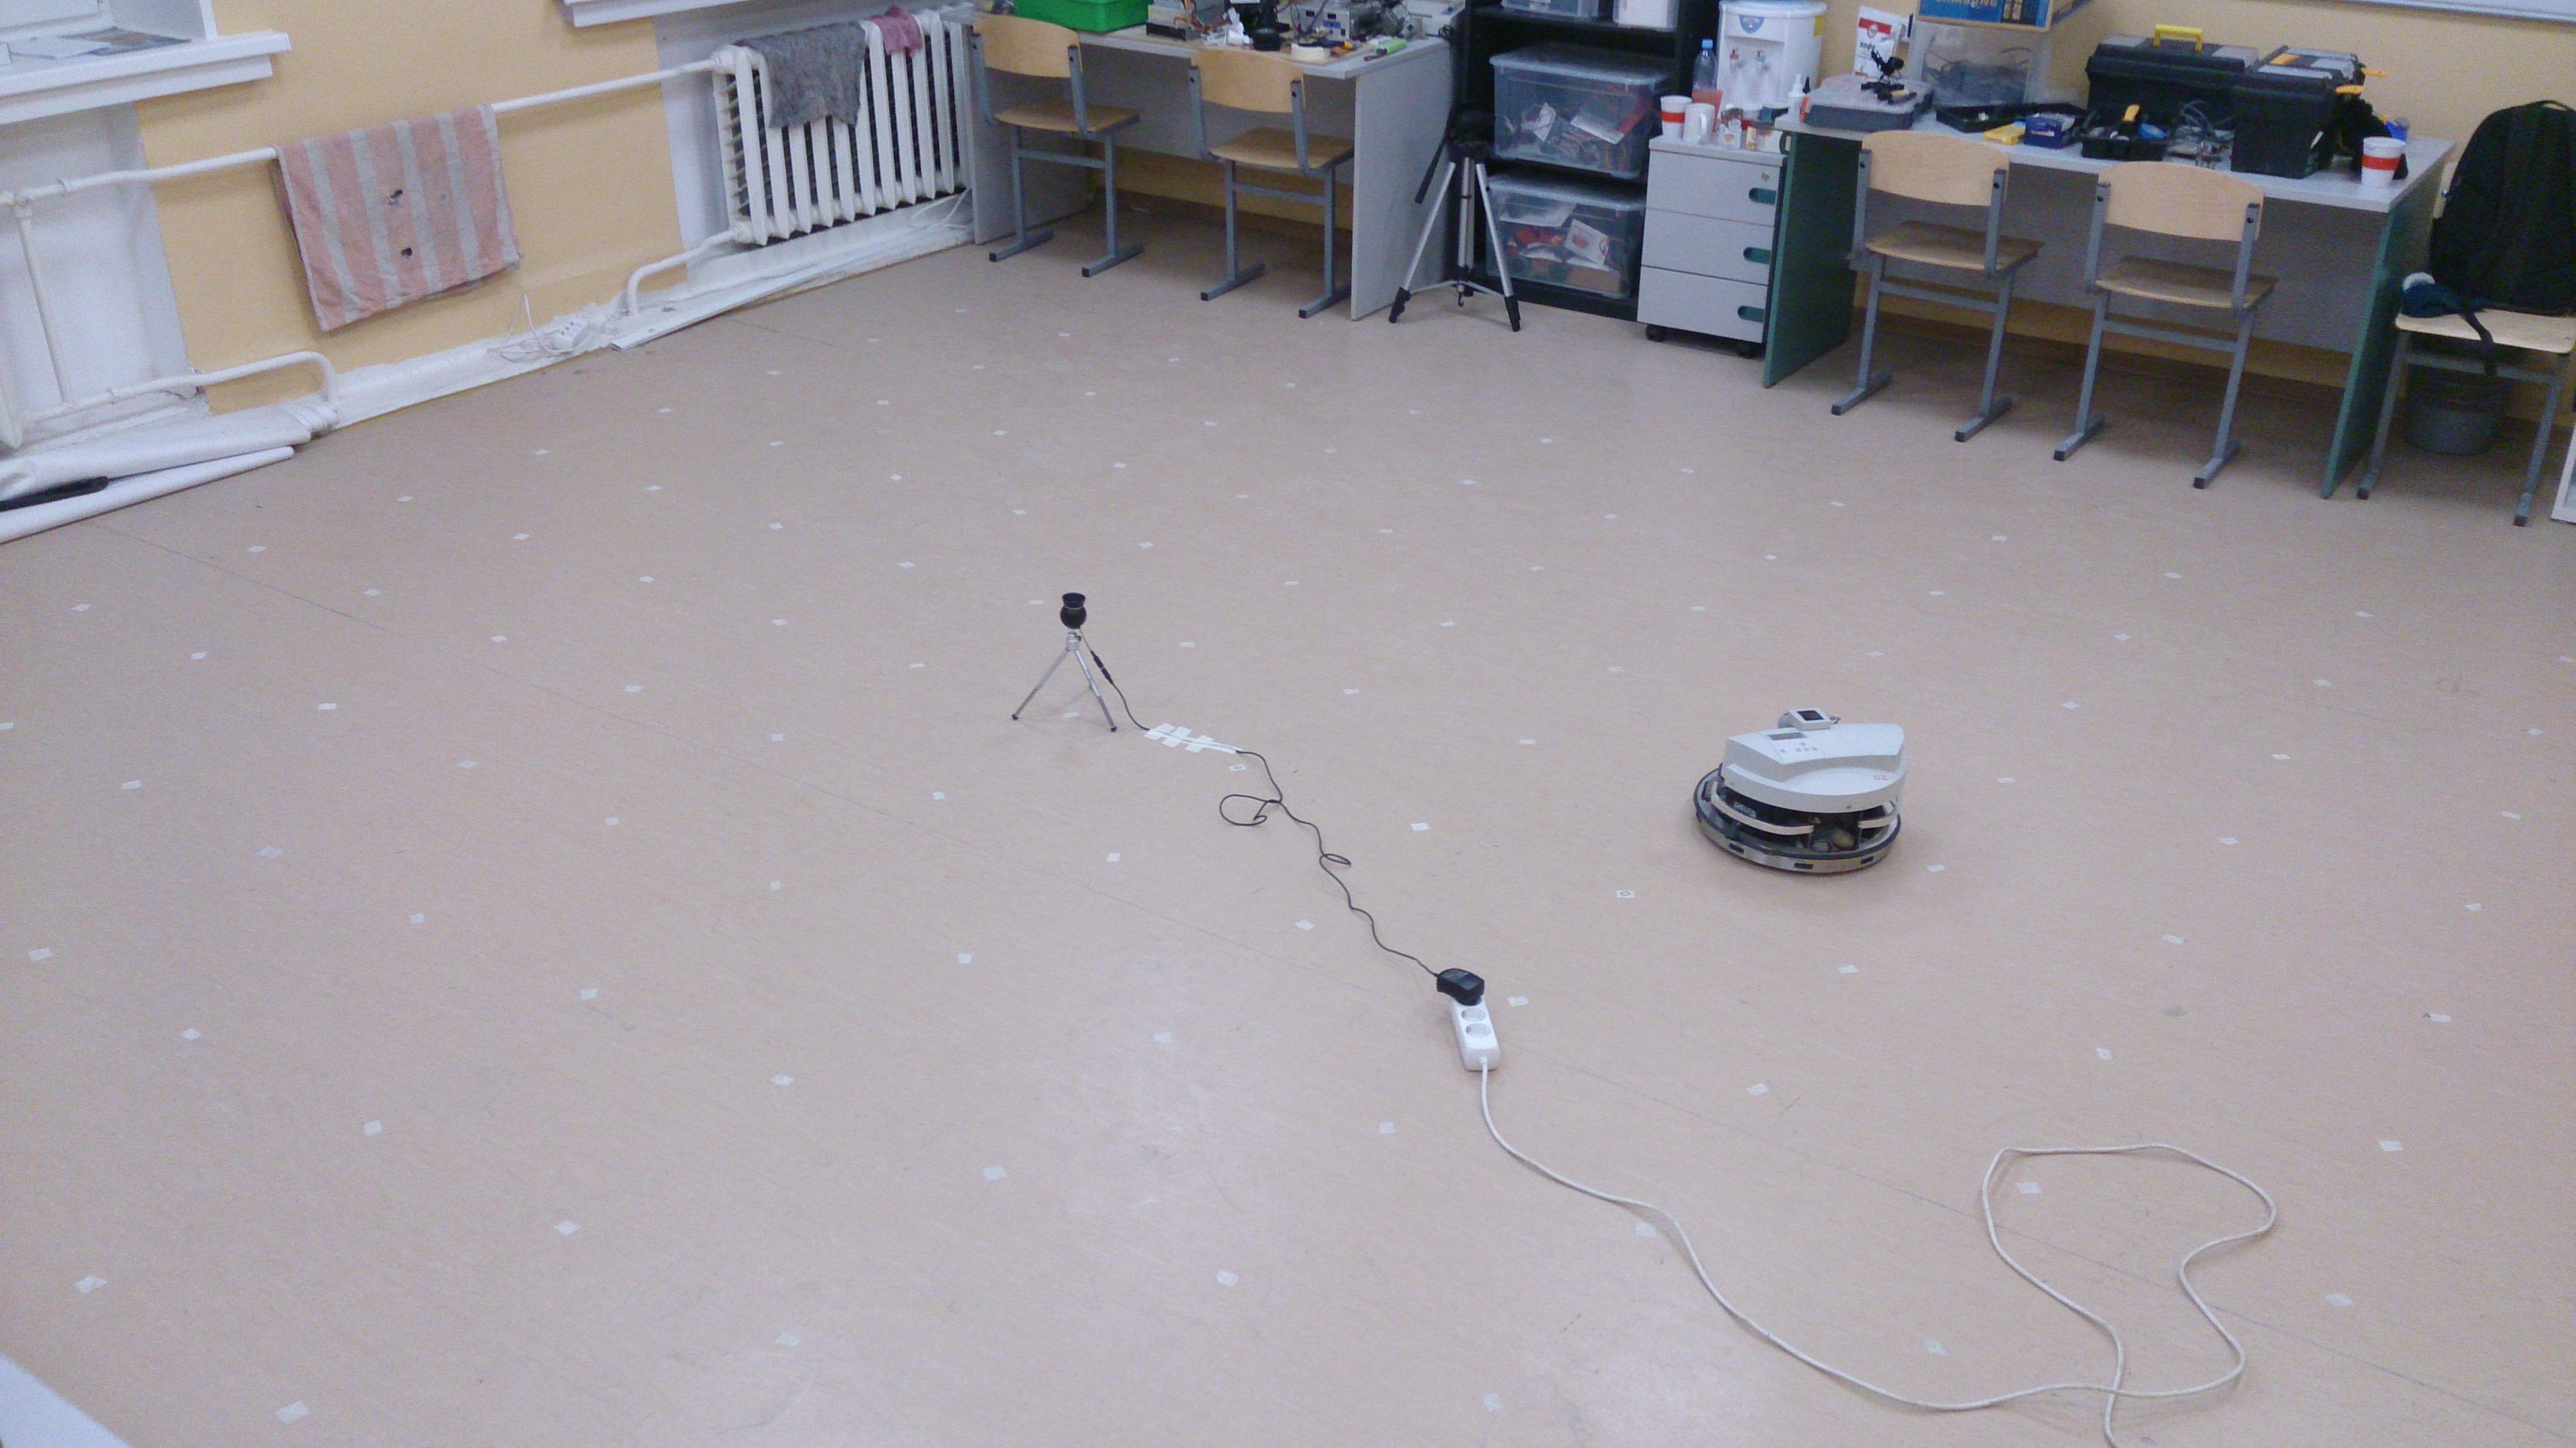
\includegraphics[width=17cm]{expers_quadro.jpg}
	\caption{Требуемая для одного из экспериментов разметка.}
	\label{img_expers_quadro}
\end{figure}

В~результате последнего действия относительно системы NorthStar были выяснены, главным образом, две вещи.

Во-первых, было установлено, что на возвращаемые ей значения сильное влияние оказывают окружающие объекты.
Это выражается в том, что, если робот, положение которого подлежит измерению, находится рядом со стеной, шкафом, столом или иным подобным предметом, показания системы NorthStar сильно искажаются.
Наглядно это демонстрирует рисунок~\ref{img_first_result_of_exps}, зелеными контурами на котором обозначены искажения в данных, вызванные близко стоящими к зоне, в которой проводился эксперимент, столами, а красным~--- искажения, вызванные находящейся в непосредственной близости к экспериментальной зоне стеной\lefteqn{.}%
\footnote{Для людей, знакомых с внутренним убранством аудитории, запечатленной на рисунке~\ref{img_expers_quadro}, во избежание недоумений с их стороны стоит сказать, что эксперимент, чьи результаты представлены на рисунке~\ref{img_first_result_of_exps}, проводился при иной расстановке мебели, нежели запечатленной на первом из обозначенных рисунков.}

\begin{figure}[h!]
	\centering
	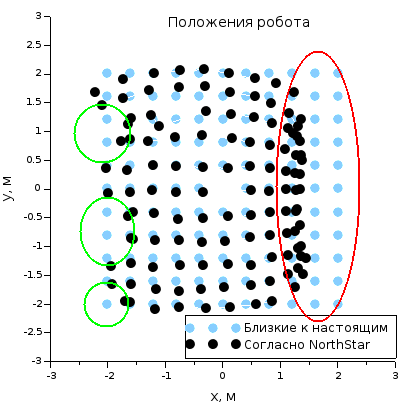
\includegraphics[height = 10cm]{errors_due_to_walls.png}
	\caption{Искажения в показаниях NorthStar, вызываемые наличием окружающих предметов.}
	\label{img_first_result_of_exps}
\end{figure}

Во-вторых было установлено, что в целом система NorthStar работоспособна.
Несмотря на то, что данные, возвращаемые системой для всей экспериментальной зоны, а она имеет размер $4{\times}4$~м, заметно искажены по краям (см.~рисунок~\ref{img_second_result_of_exps}%
\footnote{В~эксперименте, чьи результаты запечатлены на данном рисунке, проектор NorthStar был повернут на $90^\circ$ относительно того положения, в котором он находился при проведении эксперимента, соответствующего рисунку~\ref{img_first_result_of_exps}.})
ближе к центру оказываются близкими к точкам экспериментальной разметки.
Если же последние подвергнуть разным смещениям и поворотам, а потом взять из них такую пару, при которой сумма квадратов отклонений экспериментальных точек от идеальных принимает наименьшее значение, тем самым попытавшись учесть отсутствие строгого выравнивания системы СКП относительно экспериментальной разметки (см.~п.~<<\ref{item:alignment}>> последнего перечня), то результат примет еще более убедительный вид, продемонстрированный на рисунке~\ref{img_second_result_of_exps_with_hacks}.

\begin{figure}[h!]
	\centering
	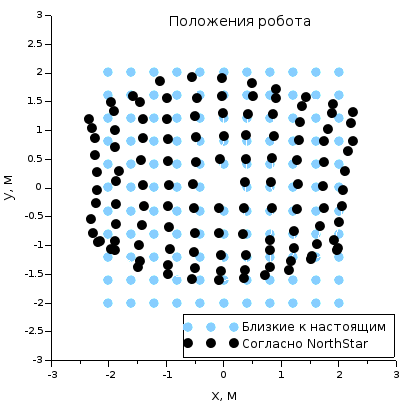
\includegraphics[height = 10cm]{quite_normal_big_ns_data.png}
	\caption{Результаты еще одного эксперимента.}
	\label{img_second_result_of_exps}
\end{figure}

\begin{figure}[h!]
	\centering
	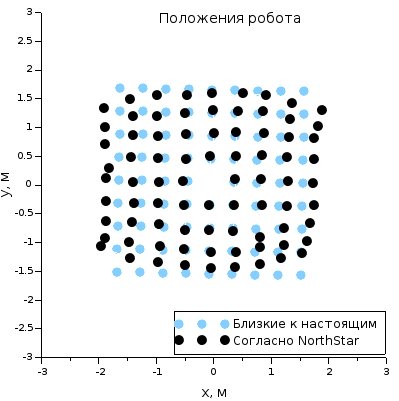
\includegraphics[height = 10cm]{ns_with_hacks.png}
	\caption{Результаты одного из экспериментов, подвергнутые постобработке.}
	\label{img_second_result_of_exps_with_hacks}
\end{figure}



\chapter{Рекомендации к дальнейшим экспериментам с NorthStar}\label{app_expers_with_ns_2}
В~данном приложении даются советы по проведению выравнивания\footnote{В~экспериментах, описанных в прошлом приложении, такое выравнивание не применялось (см.~п.~<<\ref{item:alignment}>> его последнего перечня).}
системы координат СКП и экспериментальной разметки, описанной в прошлом приложении и представляющей собой квадрат из $11{\times}11$ точек, расстояние между которыми 40~см.

Предлагаемый алгоритм следующий (предполагается доступность двух Robotino, снабженных приемниками NorthStar):
\begin{enumerate}
	\item поместить проектор Northstar, чья <<голова>> приблизительно направлена вертикально вверх, в точку 0, а обоих Robotino, снабженных приемниками в точки 1 и 3 (см.~рисунок~\ref{img_numbered_figure});
	\item перемещать проектор и изменять угол наклона его головы до тех пор, пока возвращаемые системой NorthStar координаты Robotino $(x_i; y_i)$, где $i=\overline{1,2}$ не станут согласовываться друг с другом, согласно соотношению $(x_1; y_1) = (-x_2; -y_2)$ (выполнение этого условия теоретически будет гарантировать выравнивание осей системы координат, относительно которой возвращаются координаты приемника, параллельно сторонам большого квадрата);
	\item проверить настройку, описанную в прошлом пункте, поместив обоих роботов в точки 2 и 4 (для их координат в этих точках также должно выполняться указанное выше равенство); при этом абсолютные значения всех координат, встречающихся как в этом пункте, так и в прошлом, должны совпадать.
\end{enumerate}

\begin{figure}[h!]
	\centering
	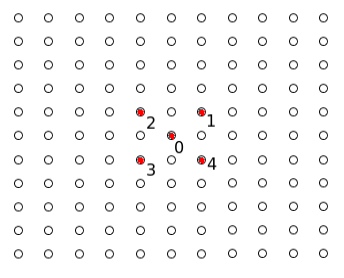
\includegraphics[height = 5.3cm]{numbered_square.png}
	\caption{Схематичное представление рассматриваемой экспериментальной разметки с необходимыми пометками.}
	\label{img_numbered_figure}
\end{figure}
